\xiti
\begin{xiaotis}

\xiaoti{求下列三角函数值:}
\begin{xiaoxiaotis}

    \xxt{$\sin{158^\circ54'} \nsep \cos{172^\circ36'} \nsep \tan{105^\circ6'} \nsep \cot{91^\circ42'}$;}

    \xxt{$\sin{136^\circ27'} \nsep \cos{118^\circ38'} \nsep \tan{155^\circ56'} \nsep \cot{142^\circ19'}$。}

\end{xiaoxiaotis}


\xiaoti{把下列各式写成锐角 $\alpha$ 或 $\beta$ 的三角函数的形式:}
\begin{xiaoxiaotis}

    \begin{tblr}{columns={18em, colsep=0pt}}
        \xxt{$\sin(180^\circ - \alpha)$;} & \xxt{$\cos(180^\circ - \beta)$;} \\
        \xxt{$\tan(90^\circ - \alpha)$;} & \xxt{$\cot(180^\circ - \beta)$。}
    \end{tblr}
\end{xiaoxiaotis}


\xiaoti{设 $A$,$B$,$C$ 为一个三角形的三个内角,求证:}
\begin{xiaoxiaotis}

    \begin{tblr}{columns={18em, colsep=0pt}}
        \xxt{$\sin(A + B) = \sin C$;} & \xxt{$\cos(B + C) = -\cos A$。}
    \end{tblr}
\end{xiaoxiaotis}


\xiaoti{求适合下列各式的三角形内角 $A$:}
\begin{xiaoxiaotis}

    \xxt{\begin{tblr}[t]{columns={8em, mode=math, colsep=0pt}, row{1}={abovesep=1em}}
        \sin{A} = \dfrac{\sqrt{2}}{2} \douhao & \cos{A} = -\exdfrac{1}{2} \douhao \\
        \tan{A} = -1 \douhao                  & \cot{A} = -\sqrt{3} \fenhao
    \end{tblr}}

    \xxt{$\sin{A} = 0.2529 \nsep \cos{A} = -0.9756 \nsep \tan{A} = -1.998$。}

\end{xiaoxiaotis}


\xiaoti{在 $\triangle ABC$ 中:}
\begin{xiaoxiaotis}

    \xxt{已知 $a = 49$, $b= 26$, $C = 107^\circ$,求 $c$,$B$;}

    \xxt{已知 $a = 84$, $b= 56$, $c = 74$,求 $A$;}

    \xxt{已知 $c = 68$, $A= 34^\circ$, $B = 56^\circ$,求 $a$ 和 $S_\triangle$。}

    \hspace*{1.5em} (本题要求角度精确到 $1^\circ$,边长、面积保留两个有效数字。)

\end{xiaoxiaotis}


\xiaoti{根据下列条件,解三角形(角度精确到 $1^\circ$,边长保留两个有效数字):}
\begin{xiaoxiaotis}

    \xxt{$b = 26 \nsep c = 15 \nsep C = 23^\circ$;}

    \xxt{$b = 54 \nsep c = 39 \nsep C = 115^\circ$。}

\end{xiaoxiaotis}


\xiaoti{从四边形操场 $ABCD$ 内的 $O$ 点,测得 $OA = 39.8$ m, $OB = 36.7$ m,
    $OC = 42.3$ m, $OD = 44.1$ m, $\angle AOB = 88^\circ$,
    $\angle BOC = 76^\circ$, $\angle COD = 102^\circ30'$,
    求这个操场的面积(保留两个有效数字)。
}

\begin{figure}[htbp]
    \centering
    \begin{minipage}[b]{7cm}
        \centering
        \begin{tikzpicture}
    \pgfmathsetmacro{\factor}{0.05}
    \pgfmathsetmacro{\oa}{39.8 * \factor}
    \pgfmathsetmacro{\ob}{36.7 * \factor}
    \pgfmathsetmacro{\oc}{42.3 * \factor}
    \pgfmathsetmacro{\od}{44.1 * \factor}
    \pgfmathsetmacro{\aob}{88}
    \pgfmathsetmacro{\boc}{76}
    \pgfmathsetmacro{\cod}{102.5}

    % 以 OA 为 x 轴负方向绘图,然后旋转一定的角度,让 BC 看起来向是水平的。
    \begin{scope}[rotate=-32] % 32度 是估计的一个值,没有计算。
        \coordinate ["$O$"] (O) at (0, 0);
        \coordinate ["$A$" left] (A) at (-\oa, 0);
        \coordinate ["$B$" left] (B) at (180+\aob:\ob);
        \coordinate ["$C$" right] (C) at (180+\aob+\boc:\oc);
        \coordinate ["$D$"] (D) at (180+\aob+\boc+\cod:\od);

        \draw (O) -- (A)
              (O) -- (B)
              (O) -- (C)
              (O) -- (D);
        \draw (A) -- (B) -- (C) -- (D) --cycle;
        \draw pic [draw, "$88^\circ$", angle radius=1.5em, angle eccentricity=1.5] {angle=A--O--B};
        \draw pic [draw, "$76^\circ$", angle radius=1.8em, angle eccentricity=1.5] {angle=B--O--C};
        \draw pic [draw, "$102^\circ30'$", angle radius=1.4em, angle eccentricity=1.4] {angle=C--O--D};
    \end{scope}
\end{tikzpicture}


        \caption*{(第 7 题)}
    \end{minipage}
    \qquad
    \begin{minipage}[b]{7cm}
        \centering
        \begin{tikzpicture}
    \pgfmathsetmacro{\factor}{0.1}
    \pgfmathsetmacro{\ac}{57 * \factor}
    \pgfmathsetmacro{\bac}{27} % \alpha
    \pgfmathsetmacro{\acb}{35} % \beta

    \pgfmathsetmacro{\abc}{180 - \bac - \acb}
    \pgfmathsetmacro{\ab}{sin(\acb) * \ac / sin(\abc)}

    \coordinate ["$A$" below] (A) at (0, 0);
    \coordinate ["$B$" below] (B) at (\ab, 0);
    \coordinate ["$C$" above] (C) at (\bac:\ac);
    \coordinate ["$D$" above] (D) at ($(C) - (\ab, 0)$);

    \draw (A) -- (B) -- (C) -- (D) -- cycle;
    \draw (A) -- (C);
    \draw pic [draw, "$\alpha$", angle radius=1.5em, angle eccentricity=1.5] {angle=B--A--C};
    \draw pic [draw, "$\beta$",  angle radius=1.8em, angle eccentricity=1.5] {angle=C--A--D};
\end{tikzpicture}



        \caption*{(第 9 题)}
    \end{minipage}
\end{figure}

\xiaoti{已知平行四边形两条邻边的长分别是 $4\sqrt{6}$ cm 和 $4\sqrt{3}$ cm,
    它们的夹角是 $45^\circ$, 求这个平行四边形的两条对角线的长和它的面积。
}


\xiaoti{如图,已知平行四边形 $ABCD$ 的对角线 $AC = 57$ cm,
    它与两条邻边 $AB$ 和 $AD$ 的夹角分别是 $\alpha = 27^\circ$ 和 $\beta = 35^\circ$,
    求 $AB$ 和 $AD$(精确到 $1$ cm)。
}

\xiaoti{为了开凿隧道,要测量隧道口 $D$,$E$ 间的距离。
    为此在山的一侧选取适当的点 $C$(如图),测得 $CA = 482.8 \, \mi$,
    $CB = 631.5 \, \mi$, $\angle ACB = 56^\circ18'$,
    又测得 $A$,$B$ 两点到隧道口的距离 $AD = 80.12 \, \mi$,$BE = 40.24 \, \mi$
    ( $A$,$D$,$E$,$B$ 在一直线上)。计算隧道 $DE$ 的长。
}

\begin{figure}[htbp]
    \centering
    \begin{minipage}[b]{7cm}
        \centering
        \begin{tikzpicture}
    \pgfmathsetmacro{\factor}{0.008}
    \pgfmathsetmacro{\ac}{482.8 * \factor}
    \pgfmathsetmacro{\bc}{631.5 * \factor}
    \pgfmathsetmacro{\ad}{80.12 * \factor}
    \pgfmathsetmacro{\be}{40.24 * \factor}
    \pgfmathsetmacro{\acb}{56.3}

    \pgfmathsetmacro{\ab}{sqrt(\ac^2 + \bc^2 - 2 * \ac * \bc * cos(\acb))}
    \pgfmathsetmacro{\abc}{asin( sin(\acb) * \ac / \ab)}

    \coordinate ["$C$" left] (C) at (0, 0);
    \coordinate ["$B$" right] (B) at (\bc, 0);
    \coordinate ["$A$" above] (A) at (\acb:\ac);
    \coordinate ["$D$" {above, xshift=0.2em, yshift=0.5em}] (D) at ($(A) + (360-\abc:\ad)$);
    \coordinate ["$E$" right] (E) at ($(B) + (180-\abc:\be)$);

    \draw [very thick] (D) -- (A) -- (C) -- (B) -- (E);
    \draw pic [draw, angle radius=1.5em] {angle=B--C--A};

    % 利用已有的 “山” 的 pic, 绘制后手工调整到(大致)与 D 点重合
    \pic [scale=0.087, rotate around=45:(E)] at (E) {mountain};
\end{tikzpicture}


        \caption*{(第 10 题)}
    \end{minipage}
    \qquad
    \begin{minipage}[b]{7cm}
        \centering
        \begin{tikzpicture}
    \pgfmathsetmacro{\factor}{0.2}
    \pgfmathsetmacro{\ab}{32.2 * 0.5 * \factor}
    \pgfmathsetmacro{\sab}{20}
    \pgfmathsetmacro{\sbc}{65}

    \coordinate ["$A$" left] (A) at (0, 0);
    \coordinate ["$B$" left] (B) at (0, \ab);
    \coordinate (C) at ($(B) + (0, 0.8)$);

    \path [name path=as] (A) -- ($(A) + (90-\sab:\ab * 1.5)$); %  \ab * 1.5 是为了让 as 和 bs 即能相交,又不会占用太多空间而选择的一个值
    \path [name path=bs] (B) -- ($(B) + (90-\sbc:\ab * 0.7)$);
    \path [name intersections={of=as and bs, by=S}];

    \draw [very thick]  (A) -- (B);
    \draw [dashed] (B) -- (C);
    \draw (A) -- (S) -- (B);
    \draw (S) circle (0.1) node [right] {$S$};
    \draw pic [draw, "$20^\circ$" {xshift=0.3em}, angle radius=2.5em, angle eccentricity=1.3] {angle=S--A--B};
    \draw pic [draw, "$65^\circ$" {xshift=0.3em}, angle radius=1.5em, angle eccentricity=1.3] {angle=S--B--C};


    \begin{scope}[xshift=1.5cm, yshift=1.5cm]
        \pgfmathsetmacro{\h}{0.5}
        \pgfmathsetmacro{\w}{0.2}
        \draw [very thick] (-\w, 0) -- (\w, 0);
        \draw [very thick] (0, -\h) -- (0, \h);
        \draw [fill=black] (-0.1, \h) -- (0.1, \h) -- (0, \h + 0.3);

        \pgfmathsetmacro{\dx}{0.1}
        \pgfmathsetmacro{\dy}{0.2}
        \pgfmathsetmacro{\dh}{0.5}
        \draw (0, -\h) -- (-\dx, -\h - \dy) -- (-\dx, -\h - \dy - \dh) -- (0, -\h - \dh) -- cycle;
        \draw [fill=black] (0, -\h) -- ( \dx, -\h - \dy) -- ( \dx, -\h - \dy - \dh) -- (0, -\h - \dh) -- cycle;
        \node at (-0.5, 0) {西};
        \node at ( 0.5, 0) {东};
        \node at (0,  1.1) {北};
        \node at (0, -1.5) {南};
    \end{scope}
\end{tikzpicture}


        \caption*{(第 11 题)}
    \end{minipage}
\end{figure}

\xiaoti{如图,一艘船以 $32.2$ 海里/时\,的速度向正北航行,在 $A$ 处看灯塔 $S$ 在船的北偏东 $20^\circ$,
    半小时后航行到 $B$ 处,在 $B$ 处看灯塔 $S$ 在船的北偏东 $65^\circ$。
    求灯塔 $S$ 和 $B$ 处的距离(精确到 $0.1$ 海里)。
}


\xiaoti{如图,在山顶铁塔上 $B$ 处测得地面上一点 $A$ 的俯角 $\alpha = 54^\circ40'$,
    在塔底 $C$ 处测得点 $A$ 的俯角 $\beta = 50^\circ1'$,已知铁塔 $BC$ 部分高 $27.3$ 米,
    求山高 $CD$ (精确到 $1$ 米)。
}

\begin{figure}[htbp]
    \centering
    \begin{minipage}[b]{7cm}
        \centering
        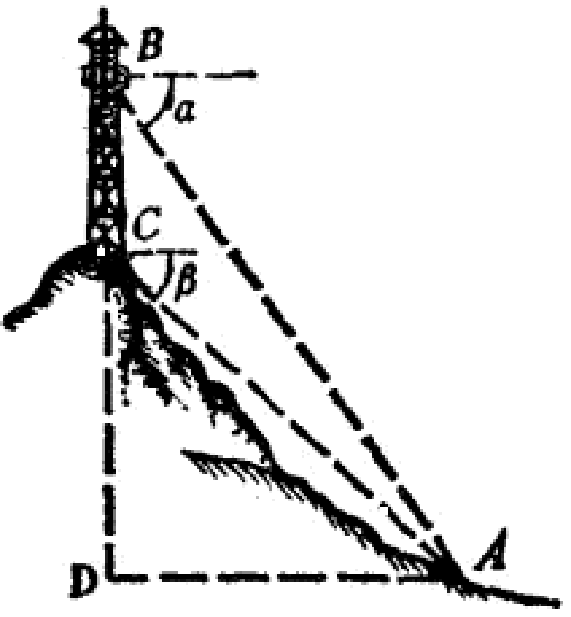
\includegraphics[width=6cm]{../pic/czds4-ch15-xiti11-12}
        \caption*{(第 12 题)}
    \end{minipage}
    \qquad
    \begin{minipage}[b]{7cm}
        \centering
        \begin{tikzpicture}[>=Stealth]
    % 各坐标点的相对位置
    %
    %   N
    %   B
    %        M  A
    %        C
    \pgfmathsetmacro{\factor}{0.3}
    \pgfmathsetmacro{\bc}{35 * 0.5 * \factor}
    \pgfmathsetmacro{\nba}{126}
    \pgfmathsetmacro{\nbc}{148}
    \pgfmathsetmacro{\mca}{78}

    \pgfmathsetmacro{\abc}{\nbc - \nba}
    \pgfmathsetmacro{\mcb}{180  - \nbc}
    \pgfmathsetmacro{\acb}{\mca + \mcb}
    \pgfmathsetmacro{\bac}{180 - \abc - \acb}
    \pgfmathsetmacro{\ac}{\bc * sin(\abc) / sin(\bac)}

    \coordinate ["$C$" below] (C) at (0, 0);
    \coordinate ["$A$" right] (A) at (90 - \mca:\ac);
    \coordinate ["$B$" left]  (B) at (90 + \mcb:\bc);

    \draw [->] (C) -- +(0, 1) coordinate (M) node [above] {北};
    \draw [->] (B) -- +(0, 1.3) coordinate (N) node [above] {北};
    \begin{scope}[every node/.style={fill=white, inner sep=1pt, outer sep=2pt},]
        \draw pic [draw, <-, "$78^\circ$", angle radius=1.5em, angle eccentricity=1.6] {angle=A--C--M};
        \draw pic [draw, <-, "$126^\circ$" {yshift=0.2em}, angle radius=2.7em, angle eccentricity=1.2] {angle=A--B--N};
        \draw pic [draw, <-, "$148^\circ$" {yshift=0.2em}, angle radius=1.2em, angle eccentricity=1.2] {angle=C--B--N};
    \end{scope}

    \draw [very thick] (A) -- (B) -- (C) -- cycle;
    \draw [dashed] (B) -- ($(B)!-0.2!(C)$);
\end{tikzpicture}


        \caption*{(第 13 题)}
    \end{minipage}
\end{figure}

\xiaoti{如图,货轮在海上以 $35$ 海里/时\,的速度沿着方位角(从指北方向顺时针转到目标方向线的水平角)
    为 $148^\circ$ 的方向航行。为了确定船位,在 $B$ 点观测灯塔 $A$ 的方位角是 $126^\circ$,
    航行半小时后到达 $C$ 点,观测灯塔 $A$ 的方位角是 $78^\circ$。
    求货轮到达 $C$ 点时与灯塔 $A$ 的距离(精确到 $1$ 海里)。
}

\end{xiaotis}

